\documentclass[12pt]{article}
\usepackage{geometry}
\usepackage{tabulary}
\geometry{a4paper,margin=1.5cm,bottom=.75cm}

\usepackage[table]{xcolor}

\usepackage{array}
\newcolumntype{L}{>{\centering\arraybackslash}m{3cm}}

\usepackage{fontawesome5}
\usepackage{ragged2e}
\usepackage{parskip}

\usepackage{booktabs,makecell,xltabular}

\usepackage[T1]{fontenc}
\usepackage[lf,default]{FiraSans}
\usepackage{zi4}

\usepackage{regexpatch}
\usepackage[os=mac]{menukeys}
\renewmenumacro{\keys}[+]{shadowedroundedkeys}
\renewmenumacro{\menu}[>]{angularmenus}
\xpatchcmd*{\SPACE}{2em}{1em}{}{}

\renewcommand{\tabularxcolumn}[1]{m{#1}}
\renewcommand{\arraystretch}{1.4}
\arrayrulecolor{gray!60!white}

\makeatletter
\renewcommand{\maketitle}{{\centering\sffamily{\LARGE\bfseries\@title}\par\vskip\baselineskip{\large\@date}\par}\vskip\baselineskip}
% nifty commands by Paul Gaborit from http://tex.stackexchange.com/a/236891/226
\def\setmenukeyswin{\def\tw@mk@os{win}}
\def\setmenukeysmac{\def\tw@mk@os{mac}}
\makeatother

\usepackage{hyperref}
\urlstyle{same}

\title{\textit{MasterFile} Description}
\author{Pedro A. S. O. Neto}
\date{Created 21 Feb, 2023}

\begin{document}

\maketitle

\emph{Documentation of MMBB\'s \textit{MasterFile}. Throughout this document, the word \textit{Task} refers to BAT, TAP, or Movement sub-batteries. Indexing starts at 1, unless specified. The word \textit{trial} refers to a single node run within the task (e.g., tap to constant beat).}

\begin{figure}[h]
\centering
\caption{Schema of the database. All information is tied by userID, which is constant for each participant, throughout all tasks and trials. For tap and movement tasks, data is split into two data frames, one containing general information about the task (i.e., time taken, howEasy, etc...), and the other containing detailed information about when taps/accelerometer readigs occur. This is done in order to avoid redundance, and researchers can merge the data frames as needed by their common keys (shown below in the black boxes).}
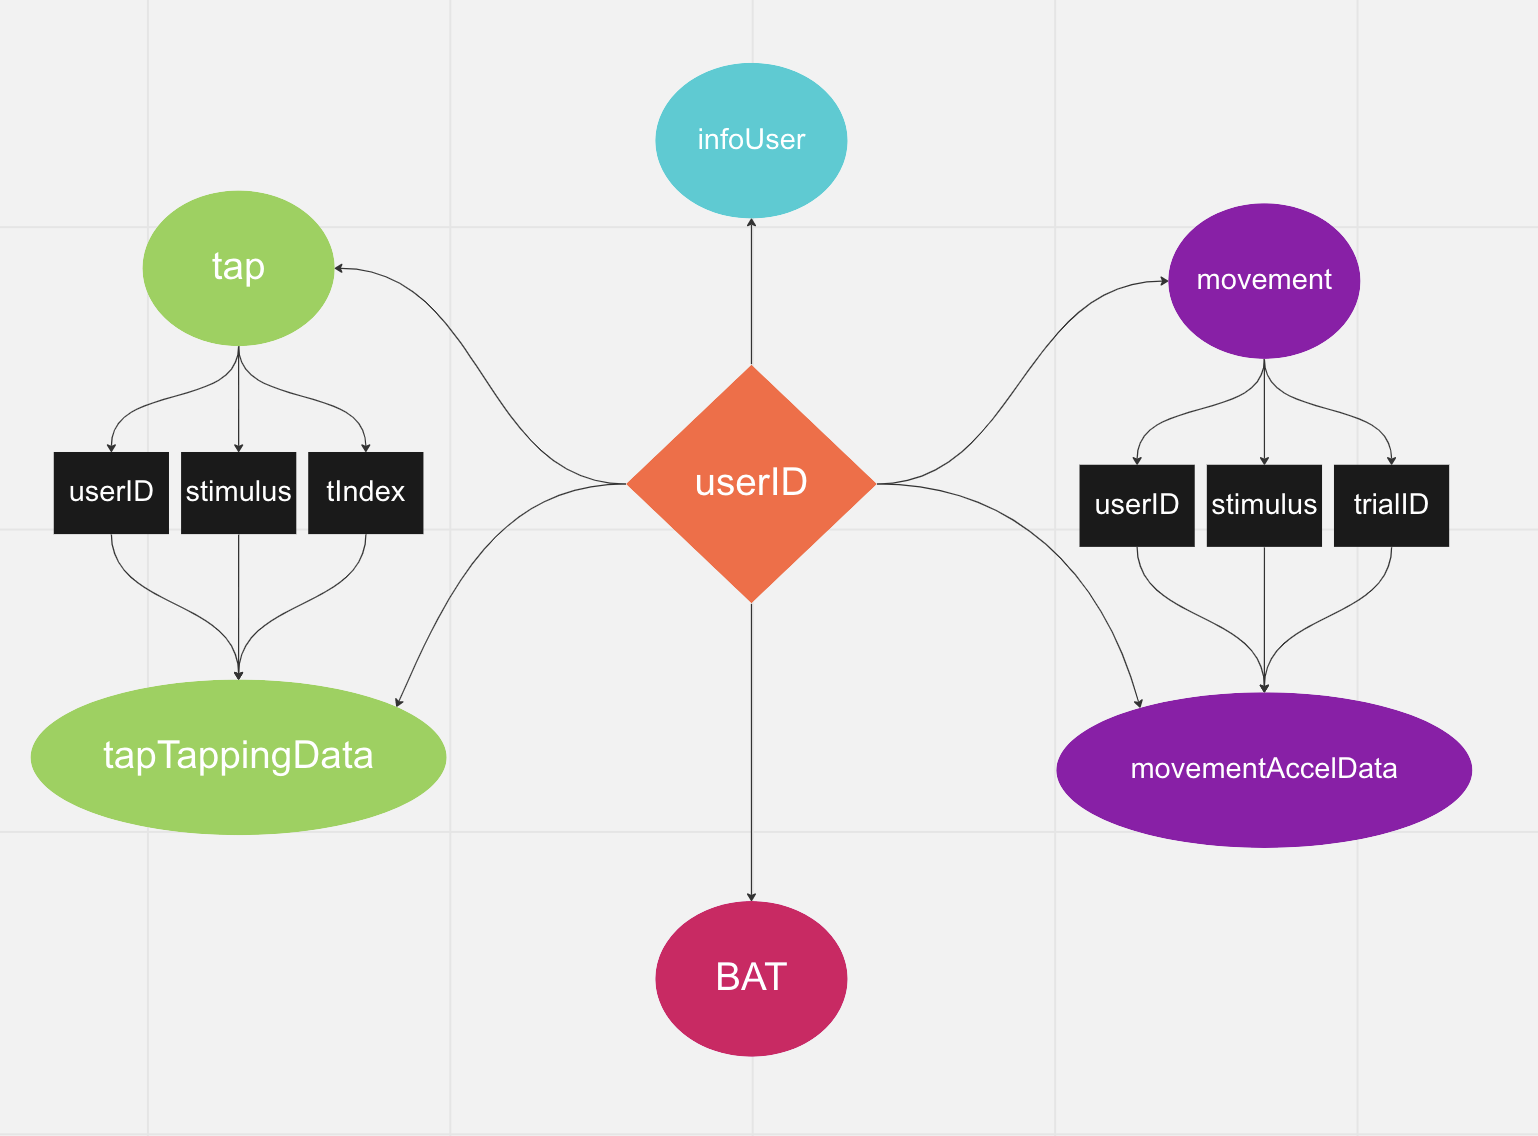
\includegraphics[width=1\textwidth]{schema.png}
\end{figure}

\bigskip

\newpage
\section{Common data} 

\emph{Data that is common to all tasks and trials}

\newline

\begin{center}
\begin{tabular}{|c|L|L|}
    \hline
    \textbf{Name} & \multicolumn{1}{m{10cm}|}{\textbf{Description}} \\
    \hline 
    
    userID & \multicolumn{1}{m{10cm}|}{Unique user identifyer}\\
    \hline

    sequenceTrials & \multicolumn{1}{m{10cm}|}{Order in which tasks (bat, tap, and movement) were presented to the participant.}\\
    \hline

    nodeIndex & \multicolumn{1}{m{10cm}|}{Index of current task within sequenceTrials (see above). If sequenceTrials equals tap,bat,movement, and nodeIndex equals 1, the current task is \textit{tap}.}\\
    \hline

    nodeName & \multicolumn{1}{m{10cm}|}{Name of current task. Always equal to sequenceTrial, at the index of nodeIndex. Redundant information, only for sannity checking.}\\
    \hline

    timeBegin & \multicolumn{1}{m{10cm}|}{Time (unix) at which participant started the current trial. Only for tapping task, timestamp indicates when the first trial is started.}\\
    \hline

    timeEnd & \multicolumn{1}{m{10cm}|}{Time (unix) at which participant finished the current trial. Only for tapping task, timestamp indicates when the last trial is finished.}\\
    \hline

    stimulus & \multicolumn{1}{m{10cm}|}{Song presented to participant in the current trial.}\\
    \hline

    outputLatencyBegin & \multicolumn{1}{m{10cm}|}{Time (s) between the browser passing an audio buffer out of an audio graph over to the host system's audio subsystem to play, and the time at which the first sample in the buffer is actually processed by the audio output device. Measured in the beginning of the trial. \href{https://developer.mozilla.org/en-US/docs/Web/API/AudioContext/outputLatency}{Web documentation}}\\
    \hline

    outputLatencyEnd & \multicolumn{1}{m{10cm}|}{Time (s) between the browser passing an audio buffer out of an audio graph over to the host system's audio subsystem to play, and the time at which the first sample in the buffer is actually processed by the audio output device. Measured in the end of the trial. \href{https://www.w3.org/TR/webaudio/#dom-audiocontext-getoutputtimestamp}{Web documentation}}\\
    \hline

\end{tabular}
\end{center}

\begin{center}
\begin{tabular}{|c|L|L|}

    \hline
    baseLatencyBegin & \multicolumn{1}{m{10cm}|}{Time (s) of processing latency incurred by the AudioContext passing the audio from the AudioDestinationNode to the audio subsystem. It does not include any additional latency that might be caused by any other processing between the output of the AudioDestinationNode and the audio hardware. Measured in the beginning of the trial. \href{https://www.w3.org/TR/webaudio/#dom-audiocontext-getoutputtimestamp}{Web Audio API official documentation}.}\\
    \hline

    baseLatencyEnd & \multicolumn{1}{m{10cm}|}{Time (s) of processing latency incurred by the AudioContext passing the audio from the AudioDestinationNode to the audio subsystem. It does not include any additional latency that might be caused by any other processing between the output of the AudioDestinationNode and the audio hardware. Measured in the end of the trial. \href{https://www.w3.org/TR/webaudio/#dom-audiocontext-getoutputtimestamp}{Web Audio API official documentation}.}\\
    \hline    
    
\end{tabular}
\end{center}

\section{Task-specific data} 

\subsection{movementAccelData} 

Accelerometer readings for each trial of the movement task.

\begin{center}
\begin{tabular}{|c|L|L|}
    \hline
    \textbf{Name} & \multicolumn{1}{m{10cm}|}{\textbf{Description}} \\
    \hline 
    
    t & \multicolumn{1}{m{10cm}|}{Time (ms) passed since the beginning of the trial until the moment at which the accelerometer measurement is taken. Javascript method: every time the \textit{devicemotion} event is triggered, \textit{performance.now()} is called and subtracted from the variable \textit{currentTrialStartTime}, declared as performance.now() at the beginning of each trial.}\\
    \hline
    
    timeAudio & \multicolumn{1}{m{10cm}|}{Time (s) of the song at which the accelerometer measurement occured, measured with \href{https://developer.mozilla.org/en-US/docs/Web/API/Web_Audio_API}{audioContext}. Javascript method: every time the \textit{devicemotion} event is triggered, \href{https://developer.mozilla.org/en-US/docs/Web/API/BaseAudioContext/currentTime}{context.currentTime} is called and subtracted from the time at which the context was created (also measured with \textit{context.currentTime}). Accuracy is automatically reduced by the browser. Use $t$ (above) as accurate measurement of time. Difference between the first $t$ and the first \textit{timeAudio} for a given track indicates when, in relation to the audio, the accelerometer started to record movement.}\\
    \hline

    x, y, z & \multicolumn{1}{m{10cm}|}{Amount of acceleration (m/s²). The acceleration value does not include the effect of the gravity force. We cannot know which axis corresponds to horizontal and vertical planes, because it depends on the position of the phone. \href{https://w3c.github.io/deviceorientation/#devicemotion}{Official documentation of devicemotion event}.}\\
    \hline

    alpha, beta, gamma & \multicolumn{1}{m{10cm}|}{Rotation rate (degrees per second) at alpha, beta, and gamma planes. \href{https://w3c.github.io/deviceorientation/#devicemotion}{Official documentation of devicemotion event}.}\\
    \hline

\end{tabular}
\end{center}

\subsection{movement} 

General information about each trial of the movement task.

\begin{center}
\begin{tabular}{|c|L|L|}

    \hline
    \textbf{Name} & \multicolumn{1}{m{10cm}|}{\textbf{Description}} \\
    \hline 

    howEasy & \multicolumn{1}{m{10cm}|}{How easy was this task for you? Scale from 0 to 100.}\\
    \hline

    howFamiliar & \multicolumn{1}{m{10cm}|}{How familiar was the song/beat to you? Scale from 0 to 100.}\\
    \hline

    groove & \multicolumn{1}{m{10cm}|}{How much did the song/beat make you want to move? Scale from 0 to 100.}\\
    \hline

    howLike & \multicolumn{1}{m{10cm}|}{How much did you like the song/beat? Scale from 0 to 100.}\\
    \hline

\end{tabular}
\end{center}


\subsection{BAT} 

General information about each trial of the BAT task.

\begin{center}
\begin{tabular}{|c|L|L|}
    \hline
    \textbf{Name} & \multicolumn{1}{m{10cm}|}{\textbf{Description}} \\
    \hline 
    
    initialOffset & \multicolumn{1}{m{10cm}|}{Initial offset between the song's beat and the underlying metronome. Offsets can be between 1 and 7, with the exception of 4. Each unit of offset translates to a quarter-note.}\\
    \hline

    offset & \multicolumn{1}{m{10cm}|}{Final offset chosen by the participant.}\\
    \hline

    nChanges & \multicolumn{1}{m{10cm}|}{Number of adjustments to the metronome offset made by participants from the beginning to the end of the trial. If nChanges == 0, offset is equal to initialOffset.}\\
    \hline

    howEasy & \multicolumn{1}{m{10cm}|}{How easy was this task for you? Scale from 0 to 100.}\\
    \hline

\end{tabular}
\end{center}

\subsection{tap} 

General information about each trial of the tapping task.

\begin{center}
\begin{tabular}{|c|L|L|}
    \hline
    \textbf{Name} & \multicolumn{1}{m{10cm}|}{\textbf{Description}} \\
    \hline 
    
    rt & \multicolumn{1}{m{10cm}|}{List of timestamps (ms) corresponsing to the time that has passed between the beginning of the trial (performance.now()), and the moment that a click/tap occured (performance.now()).}\\
    \hline

    rtAudio & \multicolumn{1}{m{10cm}|}{List of timestamps (s) corresponding to the time of the song at which the tap occured. Measured with \href{https://developer.mozilla.org/en-US/docs/Web/API/Web_Audio_API}{audioContext}. Javascript method: every time the \textit{click} event is triggered, \href{https://developer.mozilla.org/en-US/docs/Web/API/BaseAudioContext/currentTime}{context.currentTime} is called and subtracted from the time at which the context was created (also measured with \textit{context.currentTime}).}\\
    \hline

\end{tabular}
\end{center}

\subsection{tapTappingData} 

Timing at which taps occured within each trial.

\begin{center}
\begin{tabular}{|c|L|L|}

    \hline
    rt & \multicolumn{1}{m{10cm}|}{List of timestamps (ms) corresponsing to the time that has passed between the beginning of the trial (performance.now()), and the moment that a click/tap occured (performance.now()).}\\
    \hline

    rtAudio & \multicolumn{1}{m{10cm}|}{List of timestamps (s) corresponding to the time of the song at which the tap occured. Measured with \href{https://developer.mozilla.org/en-US/docs/Web/API/Web_Audio_API}{audioContext}. Javascript method: every time the \textit{click} event is triggered, \href{https://developer.mozilla.org/en-US/docs/Web/API/BaseAudioContext/currentTime}{context.currentTime} is called and subtracted from the time at which the context was created (also measured with \textit{context.currentTime}).}\\
    \hline

\end{tabular}
\end{center}

\end{document}
